\documentclass{article}
% \documentclass{beamer}
% \usetheme{Madrid}


%------------------------------

\usepackage{fancyhdr} % Set up page numbering, and make included tex files consistent
% Set up page numbering
\pagestyle{fancy}
\fancyhf{} % Clear header and footer
\rfoot{\thepage} % Right-aligned page number


% used to include other .tex files
\usepackage{standalone}

% for symbols like degree
\usepackage{gensymb}  

% used for href/url
\usepackage{hyperref}


% used for math fomulas
\usepackage{amsmath}

% used for pictures
\usepackage{graphicx}
\usepackage{subcaption}
\usepackage{float}

% used for tables
\usepackage{booktabs} % For better looking tables

% used for codes
\usepackage{listings}
\lstset{
  basicstyle=\ttfamily\footnotesize, % Set your code to be drawn with a monospaced font
  breaklines=true, % Enables line breaking
  frame=single % Adds a frame around the code
}

% used for Graph
\usepackage{adigraph}

% used for Bayesian Network
\usepackage{tikz}
\usetikzlibrary{bayesnet}

%------------------------------
% TODO 
\tolerance=10000
\emergencystretch=\maxdimen
\hyphenpenalty=10000
\hbadness=10000


\usepackage{silence}
\WarningFilter{latex}{Overfull \hbox}

%------------------------------



\title{MK's Notes for \\ CIVL-4530/6970 Geometric Design}
\date{2024-03-04}
\author{Michael Chen}

\begin{document}
  \pagenumbering{gobble}
  \maketitle

  \begin{align*}
  \\
  \\
  \\
  \\
  \\
  \\
  \\
  \\
  & \text{Geometric design is the base of transportation,}\\ 
  \\
  & \text{providing fundamental concepts, terms, and fomulas.}\\
  \end{align*}
  \newpage
  \pagenumbering{arabic}
  % \setcounter{page}{0}

  % todo ----------------------------------------
  \tableofcontents
  \newpage


  % include all chapters
  \documentclass{article}
% \documentclass{beamer}
% \usetheme{Madrid}

%------------------------------
% used for href/url
\usepackage{hyperref}


% used for math fomulas
\usepackage{amsmath}

% used for pictures
\usepackage{graphicx}
\usepackage{subcaption}
\usepackage{float}

% used for codes
\usepackage{listings}
\lstset{
  basicstyle=\ttfamily\footnotesize, % Set your code to be drawn with a monospaced font
  breaklines=true, % Enables line breaking
  frame=single % Adds a frame around the code
}

% used for Graph
\usepackage{adigraph}

% used for Bayesian Network
\usepackage{tikz}
\usetikzlibrary{bayesnet}

%------------------------------
% TODO 
\tolerance=10000
\emergencystretch=\maxdimen
\hyphenpenalty=10000
\hbadness=10000


\usepackage{silence}
\WarningFilter{latex}{Overfull \hbox}

%------------------------------



\title{MK's Notes for CIVL-4530 Geometric Design}
\date{2024-03-04}
\author{Michael Chen}

\begin{document}
  \pagenumbering{gobble}
  \maketitle
  \newpage
  \pagenumbering{roman}


  % ----------------------------------------
  \tableofcontents
  \newpage


  % ----------------------------------------
  Geometric Design is a basic course of Transportation, introducing principal concepts and fomulas.

  \newpage

  % ----------------------------------------
  \setcounter{section}{0}
  \section{Chapter 01 Introduction and Highway Function}
  \subsection{Objectives}
  \begin{enumerate}
    \item Geometric Design concepts
    \item Highway Funciton
  \end{enumerate}

  \subsection{Geometric Design Definition}
  \begin{enumerate}
    \item fit the highway to the terrain
    \item maintaining design standards for safety and performance
  \end{enumerate}

  \subsection{Geometric Design Basic}
  \begin{enumerate}
    \item make criteria matches  
    \begin{enumerate}
      \item driver expectancy/behavior
      \item vehicle performance/behavior
    \end{enumerate}
    \item balance safty, cost, mobility, community values, environmental, politics, liability, sustainable development, etc
  \end{enumerate}

  \subsection{AASHTO Role}
  \begin{enumerate}
    \item American Association of State Highway and Transportation Officials
    \item the membership of AASHTO consists of FHWA, and state DOTs
  \end{enumerate}

  % ----------------------------------------
  \subsection{Reference - AASHTO publications}
  \begin{enumerate}
    \item \textbf{a.k.a Green Book/PGDHS:} A Policy on Geometric Design of Highways and Streets, 2018, 7th Edition
    \item Guidelines for Geometric Design of Very Low Volume Local Roads, 2001
    \item A Guide to Achieving Flexibility in Highway Design, May 2004
    \item Guide for the Planning, Design, and Operation of Pedestrian Facilities, July 2004
    \item Guide for the Development of Bicycle Facilities, June 2012

    \item Good for New Highway Design 
    \item TRB Special Report 214, Designing Safer Roads: Practices for Resurfacing, Restoration, and Rehabilitation for guidance. \\
  \end{enumerate}

  \subsection{Reference - ITE publications}
  \begin{enumerate}
    \item Urban Street Geometric Design Handbook, 2008
    \item Freeway and Interchange Geometric Design Handbook, 2007
    \item Designing Walkable Urban Thoroughfares: A Context Sensitive Approach, March 2010
  \end{enumerate}

  % ------------------ todo

  \subsection{Older Driver Deficiencies}


  \begin{tabular}{|c|c|c|c|c|}
    Roadway & urban & rural level & rural rolling & rural mountainous\\
    \hline
    Freeway & C/D   & B & B & C\\
    Arterial & C/D  & B & B & C\\
    Collector & D   & C & C & D\\
    Local & D       & D & D & D\\
  \end{tabular}
  \begin{figure}[h!]
    \includegraphics[width=\linewidth]{LOS.png}
    \caption{Level of Service}
    \label{fig:image-LOS}
  \end{figure}

  \subsection{13 AASHTO Criteria}
  \begin{enumerate}
      \item design speed
      \item lane width
      \item shoulder width
      \item bridge width
      \item structural capacity
      \item 
      \item horizontal alignment
      \item vertical alignment
      \item cross slope
      \item grades
      \item superelevation
      \item horizontal clearance
      \item vertical clearance
  \end{enumerate}

  \subsection{speed}
  \begin{enumerate}
    \item running speed - the speed of an individual vehicle
    \item design speed - AASHTO: max safe speed
    \item operation speed - the 85th percentile of observed speed in free flow conditions
    \item safty of over speed - $\Delta$V: [0, 5] low; [5, 15] medium; [15, infinit] high
  \end{enumerate}

  minimum design speed for \textbf{rural} roadways vs vehicle per day(VPD)
  \begin{tabular}{|c|c|c|c|}
    \hline
    rural terrain & 0-400 & 400-2000 & over 2000 \\
    \hline
    level         & 40    & 50       & 60 \\
    rolling       & 30    & 40       & 50 \\
    mountainous   & 20    & 30       & 40 \\
  \end{tabular}

  \subsection{lane width for urban and rural (1-2ft wider than urban)}
  \begin{tabular}{|l|l|l|}
    Types & urban & rural \\
    \hline
    Freeway and Interstates: & 12ft, & 12ft\\
    Ramp: & 12-30ft & 12-30ft \\ 
    Arterial: & 11-12ft, & 10-12ft \\
    Collections: & 10-12ft, & 10-12ft\\
    local roads: & 9-12ft, & 9-12ft  \\
  \end{tabular}

  \subsection{cross slope}
  paved surfaces: 1.5-2\%, typical 2\%  - Green Book\\
  unpaved surfaces: 2-6\% - Green Book\\
  areas with high intensity rainfall: 2-2.5\% \\
  ALDOT use in 2 Counties: 2.2\% \\



\begin{table}[ht]
\centering
\caption{Lane Widths for Different Types of Roadways}
\label{tab:lane_widths}
\begin{tabular}{@{}lcccc@{}}
\hline
\textbf{Type of Roadway} & \multicolumn{2}{c}{\textbf{Rural}} & \multicolumn{2}{c}{\textbf{Urban}} \\
                         & \textbf{US (feet)} & \textbf{Metric (meters)} & \textbf{US (feet)} & \textbf{Metric (meters)} \\ 
\hline
Freeway                  & 14-16*             & 4.3-4.9*                & 14–16*             & 4.3–4.9*                \\
Arterial                 & 14-16              & 4.3-4.9                 & 14–16              & 4.3–4.9                 \\
Collector                & 14                 & 4.3                     & 14                 & 4.3                     \\
Local                    & 14                 & 4.3                     & 14                 & 4.3                     \\
\hline
\end{tabular}
\end{table}




\begin{table}[ht]
\centering
\caption{Functional Classification of Roadways}
\label{tab:functional_classification}
\begin{tabular}{@{}lccc@{}}
\hline
\textbf{Criteria} & \textbf{Local} & \textbf{Collector} & \textbf{Arterial} \\
\hline
Street pavement width & 24 ft & 22 ft (1), 31 ft & 36 ft (2), 48 ft \\
Minimum horizontal curve radius & 200 ft & 350 ft & 550 ft \\
Maximum grade (3) & 15\% & 12\% & 8\% \\
Minimum design speed for vertical curve & 25 mi/h & 35 mi/h & 45 mi/h \\
\hline
\end{tabular}
\end{table}


  % ----------------------------------------
  \subsection{Terms}
  SU - represents all single unit trucks and small buses, with length 35-60ft \\
  ADT - average daily traffic \\
  AADT - the annual average daily traffic, empersizing annual average \\
  DHV - design hour volume \\
  DDHV - The directional design hour volume \\
  30HV - the 30th Highest Hour of Yearly Traffic - the 30th Hour volume \\
  design speed (DS) - design maximum speed of a roadway \\
  free flow speed (FFS) - the observed speed at which vehicles can travel with minimal delays and no restrictions from traffic signals, congestion, or other factors. \\
  LOS - Characterization of operating conditions, related to speed, travel time, traffic density, freedom to maneuver  \\
  FFS is close to DS - It means a good design \\
  K-factor - DHV = K * ADT, K is 8 to 12\% for urban facilities; 12 to 18\% for rural facilities.  \\
  D-factor - DDHV = D * DHV, D is 50\% for urban highways; 55 - 80\% for rural and suburban roads \\
  DDHV = ADT (or AADT) * K * D \\
  CMF - Crash Modification Factor \\
  Cul-de-sac: deed end street \\

  \subsection{Rules}
  Tandem Axle - 2 axles which are very close\\
  State maximum gross vehicle weight - 73,280 - 164,000 lbs\\
  State maximum gross vehicle weight - 73,280 - 164,000 lbs\\
  \\
  DHV = 8\% - 12\% ADT in urban area, refer to Green Book\\
  30HV = 15\% ADT in a typical rural arterial, refer to Green Book\\

  % ----------------------------------------
  \subsection{Formulas}
  1 mile = 5,280 feet \\
  1000 kg = 2204.62 lbs \\
  1 foot = 0.3048 meters \\
  1 lb = 16 oz \\
  1 gallon = 3.785 liters (U.S. liquid gallon) \\
  1 gallon = 4.546 liters (U.K. imperial gallon) \\


  % ----------------------------------------
  \subsection{Reference}
  FHWA Website \\
  http://safety.fhwa.dot.gov/geometric/pubs/mitigationstrategies/ \\

  \newpage

  % ----------------------------------------
  \section{Writing Formulas}
  \subsection{Equation - ONLY support one formula per line}
  \begin{equation}
    formula 1: f(x) = x^2   ----
    formula 2: \prod_{2}^{n}
  \end{equation}

  \subsection{Align - support MULTIPLE formulas in the same block}
  NOTE: need use package amsmath to enable Align 
  \begin{align*}
    f(x) &= x & 2 \\
    g(x) &= \frac{1}{x} \\
    F(x) = f(x) + g(x) &= \int_{a}^{b} \frac{1}{3}x^3 \\
    W(x) &= \frac{1}{\sqrt{x}} + \frac{1}{\sqrt[3]{y}} \\
    Z(x) &= \left( 3 + 2 \right) * 2
  \end{align*}
  \subsubsection{}
  So which one, align or equation, will you use?


  \subsection{Inline math}
  The form is used for $ f(x) = x^ 2 $ or $\lambda$, so you can easily to use them. 
  https://github.com/LucaCappelletti94/adigraph
  \subsection{Matrics}
  $
  \left[
  \begin{matrix}
    3 & 2 \\
    9 & 4 & x
  \end{matrix}
  \right]
  $

  \newpage


  % ----------------------------------------
  \section{Embedding Pictures/Figures}

  \subsection{One figure}
  NOTE: need to use package graphicshttps://github.com/LucaCappelletti94/adigraph to enable figure

  \begin{figure}[h!]
    % \includegraphics[width=\linewidth]{}
    \caption{Auburn Campus}
    \label{fig:au01}
  \end{figure}

  \subsection{Multiple figures}
  NOTE: need to use package subcaption to enable Multiple figures.
  Here are figures:
  \begin{figure}[H]
    \centering
    \begin{subfigure}[b]{0.4\linewidth}
      % \includegraphics[width=\linewidth]{}
      \caption{Auburn Overview}
    \end{subfigure}
    \begin{subfigure}[b]{0.4\linewidth}
      % \includegraphics[width=\linewidth]{}
      \caption{Auburn Buildings}
    \end{subfigure}
    \caption{Two Auburn Old Pictures}
    \label{fig:twoPic}
  \end{figure}

  \subsection{Use float and H}
  Use package float and attribute H to strictly fix the pictures' posisiton to HERE.

  \begin{lstlisting}[caption={An Example}]
    \usepackage{float}
    ...


    \begin{figure}[H]
      ....
    \end{figure}

    
  \end{lstlisting}
  \newpage


  % ----------------------------------------

  \section{Drawing Bayesian Network and Graph}
  \subsection{Use pagckages: tikz and bayesnet}
  Use 2 packages: tikz and bayesnet to draw Bayesian Network chat.
  \break

  Type 1:
  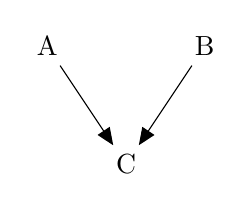
\begin{tikzpicture}
  \node (A) at (0,0) {A};
  \node (B) at (2,0) {B};
  \node (C) at (1,-1.5) {C};
  \draw[->] (A) -- (C);
  \draw[->] (B) -- (C);
  \end{tikzpicture}


  Type 2:
  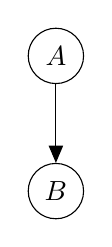
\begin{tikzpicture}
  \node[latent] (A) {$A$};
  \node[latent, below = of A] (B) {$B$};
  \edge {A} {B};
  \end{tikzpicture}
  \iffalse
  \fi
  
 
  \subsection{Use pagckages: adigraph}

  \NewAdigraph{myAdigraph}{
    s:0,0;
    1:2,2;
    3:2,-2;
    2:6,2;
    4:6,-2;
    t:8,0;
}{
    s,1:25;
    s,3:25;
    3,4:25;
    1,2:35;
    2,t:20;
    4,t:30;
    3,1:10;
    4,2:10;
    2,3:15::near start;
    4,1:5::near start;
}
\myAdigraph{}

\newpage


% --------------------------------------
\section{Using packages}
Packages are like plugins to extend the Latex' capabilities. Some common commands are listed here.

\begin{lstlisting}[language=bash, caption={tlmgr commands and etc}]
tlmgr list --only-installed   # show installed packages

tlmgr search <package-name>   # search a packages
tlmgr info <package-name>     # show a package's intro, no matter installed or not
tlmgr install <package-name>  # install a new packages

tlmgr update --self --all     # update package index

kpsewhich article.sty         # locate a package's .sty file

# env variables can define additional directories to be searched. 
echo $TEXMFHOME $TEXMFLOCAL $TEXMFSYSCONFIG 
\end{lstlisting}
\newpage


% --------------------------------------
\section{Generate Slides}
Use the package beamer to generate a pdf file of slides from an article


\begin{lstlisting}[caption={Changes in .tex file}]
  % \documentclass{article}
  \documentclass{beamer}
  \usetheme{Madrid}
\end{lstlisting}

% --------------------------------------
\end{document}
  \newpage
  \documentclass{article}
% \documentclass{beamer}
% \usetheme{Madrid}

%------------------------------
% used for href/url
\usepackage{hyperref}


% used for math fomulas
\usepackage{amsmath}

% used for pictures
\usepackage{graphicx}
\usepackage{subcaption}
\usepackage{float}

% used for codes
\usepackage{listings}
\lstset{
  basicstyle=\ttfamily\footnotesize, % Set your code to be drawn with a monospaced font
  breaklines=true, % Enables line breaking
  frame=single % Adds a frame around the code
}

% used for Graph
\usepackage{adigraph}

% used for Bayesian Network
\usepackage{tikz}
\usetikzlibrary{bayesnet}

%------------------------------
% TODO 
\tolerance=10000
\emergencystretch=\maxdimen
\hyphenpenalty=10000
\hbadness=10000


\usepackage{silence}
\WarningFilter{latex}{Overfull \hbox}

%------------------------------



\title{MK's Notes for CIVL-4530 Geometric Design}
\date{2024-03-04}
\author{Michael Chen}

\begin{document}
  \pagenumbering{gobble}
  % \maketitle
  % \newpage
  \pagenumbering{arabic}
  % \setcounter{section}{1}


  % todo ----------------------------------------
  % \tableofcontents
  % \newpage


  % ----------------------------------------
  \section{Design Control and Criteria}
  \subsection{Objectives}
  \begin{enumerate}
    \item Design Vehicles, Driver and Traffic Characteristics
    \item 13 AASHTO criteria
    \item AASHTO administered, federal-wide
    \item State-DOT administered - Green Book
    \item local goverment administered - ordinance or code
  \end{enumerate}

  \subsection{Design vehicles}
  \begin{enumerate}
    \item Design Vehicle\\ 
    Its weight, dimensions, and operating characteristics will be used to establish the geometric standards of the highway.
    \item design vehicle P: passenger car
    \begin{enumerate}
      \item Geometry - length 19ft (5+11+3), width 7ft
      \item Minimum turning path - outline 25.4ft, front wheel 23.8ft, CTR 21ft, min 14.4ft 
    \end{enumerate}
    \item WB-50 - length 55ft, width 8.5ft, height 13.5ft
  \end{enumerate}

  ASSHTO guideline - Selection of design vehicle \ref{fig:image-design-vehicles}
  \begin{figure}[!ht]
    \includegraphics[width=0.7\linewidth]{design-vehicles.png}
    \caption{Design Vehicles}
    \label{fig:image-design-vehicles}
  \end{figure}
  \begin{enumerate}
    \item parking lot - passenger car
    \item intersection of local area - SU-30, 30ft
    \item intersection of state highway and city street - City transit buses, 40ft
    \item intersections of highways; low-volume county roads with ADT < 400 - City bus (40ft, 84 passengers) or conventional bus(36ft, 64 passengers)
    \item freeway ramp; arterial crossroads; intersections of state highways; with high volume of traffic - WB-40 to WB-62
  \end{enumerate}

  \subsection{Older Driver Deficiencies}
  \begin{enumerate}
    \item Slower information processing
    \item Slower reaction times
    \item Slower decision making
    \item Visual deterioration
    \item Hearing deterioration
    \item Decline in ability to judge time, speed, and distance
    \item Limited depth perception
    \item Limited physical mobility
    \item Side effects from prescription drugs
  \end{enumerate}

  \subsection{LOS and ADT}
  acceptable LOS / level of "congestion" \ref*{fig:image-LOS} \\

  \begin{tabular}{|c|c|c|c|c|}
    Roadway & urban & rural level & rural rolling & rural mountainous\\
    \hline
    Freeway & C/D   & B & B & C\\
    Arterial & C/D  & B & B & C\\
    Collector & D   & C & C & D\\
    Local & D       & D & D & D\\
  \end{tabular}
  \begin{figure}[h!]
    \includegraphics[width=\linewidth]{LOS.png}
    \caption{Level of Service}
    \label{fig:image-LOS}
  \end{figure}

  \subsection{13 AASHTO Criteria}
  \begin{enumerate}
      \item design speed
      \item lane width
      \item shoulder width
      \item bridge width
      \item structural capacity
      \item 
      \item horizontal alignment
      \item vertical alignment
      \item cross slope
      \item grades
      \item superelevation
      \item horizontal clearance
      \item vertical clearance
  \end{enumerate}

  \subsection{speed}
  \begin{enumerate}
    \item running speed - the speed of an individual vehicle
    \item design speed - AASHTO: max safe speed
    \item operation speed - the 85th percentile of observed speed in free flow conditions
    \item safty of over speed - $\Delta$V: [0, 5] low; [5, 15] medium; [15, infinit] high
  \end{enumerate}

  minimum design speed for \textbf{rural} roadways vs vehicle per day(VPD)
  \begin{tabular}{|c|c|c|c|}
    \hline
    rural terrain & 0-400 & 400-2000 & over 2000 \\
    \hline
    level         & 40    & 50       & 60 \\
    rolling       & 30    & 40       & 50 \\
    mountainous   & 20    & 30       & 40 \\
  \end{tabular}

  \subsection{lane width for urban and rural (1-2ft wider than urban)}
  \begin{tabular}{|l|l|l|}
    Types & urban & rural \\
    \hline
    Freeway and Interstates: & 12ft, & 12ft\\
    Ramp: & 12-30ft & 12-30ft \\ 
    Arterial: & 11-12ft, & 10-12ft \\
    Collections: & 10-12ft, & 10-12ft\\
    local roads: & 9-12ft, & 9-12ft  \\
  \end{tabular}

  \subsection{cross slope}
  paved surfaces: 1.5-2\%, typical 2\%  - Green Book\\
  unpaved surfaces: 2-6\% - Green Book\\
  areas with high intensity rainfall: 2-2.5\% \\
  ALDOT use in 2 Counties: 2.2\% \\



\begin{table}[ht]
\centering
\caption{Lane Widths for Different Types of Roadways}
\label{tab:lane_widths}
\begin{tabular}{@{}lcccc@{}}
\hline
\textbf{Type of Roadway} & \multicolumn{2}{c}{\textbf{Rural}} & \multicolumn{2}{c}{\textbf{Urban}} \\
                         & \textbf{US (feet)} & \textbf{Metric (meters)} & \textbf{US (feet)} & \textbf{Metric (meters)} \\ 
\hline
Freeway                  & 14-16*             & 4.3-4.9*                & 14–16*             & 4.3–4.9*                \\
Arterial                 & 14-16              & 4.3-4.9                 & 14–16              & 4.3–4.9                 \\
Collector                & 14                 & 4.3                     & 14                 & 4.3                     \\
Local                    & 14                 & 4.3                     & 14                 & 4.3                     \\
\hline
\end{tabular}
\end{table}




\begin{table}[ht]
\centering
\caption{Functional Classification of Roadways}
\label{tab:functional_classification}
\begin{tabular}{@{}lccc@{}}
\hline
\textbf{Criteria} & \textbf{Local} & \textbf{Collector} & \textbf{Arterial} \\
\hline
Street pavement width & 24 ft & 22 ft (1), 31 ft & 36 ft (2), 48 ft \\
Minimum horizontal curve radius & 200 ft & 350 ft & 550 ft \\
Maximum grade (3) & 15\% & 12\% & 8\% \\
Minimum design speed for vertical curve & 25 mi/h & 35 mi/h & 45 mi/h \\
\hline
\end{tabular}
\end{table}


  % ----------------------------------------
  \subsection{Terms}
  SU - represents all single unit trucks and small buses, with length 35-60ft \\
  ADT - average daily traffic \\
  AADT - the annual average daily traffic, empersizing annual average \\
  DHV - design hour volume \\
  DDHV - The directional design hour volume \\
  30HV - the 30th Highest Hour of Yearly Traffic - the 30th Hour volume \\
  design speed (DS) - design maximum speed of a roadway \\
  free flow speed (FFS) - the observed speed at which vehicles can travel with minimal delays and no restrictions from traffic signals, congestion, or other factors. \\
  LOS - Characterization of operating conditions, related to speed, travel time, traffic density, freedom to maneuver  \\
  FFS is close to DS - It means a good design \\
  K-factor - DHV = K * ADT, K is 8 to 12\% for urban facilities; 12 to 18\% for rural facilities.  \\
  D-factor - DDHV = D * DHV, D is 50\% for urban highways; 55 - 80\% for rural and suburban roads \\
  DDHV = ADT (or AADT) * K * D \\
  CMF - Crash Modification Factor \\
  Cul-de-sac: deed end street \\

  \subsection{Rules}
  Tandem Axle - 2 axles which are very close\\
  State maximum gross vehicle weight - 73,280 - 164,000 lbs\\
  State maximum gross vehicle weight - 73,280 - 164,000 lbs\\
  \\
  DHV = 8\% - 12\% ADT in urban area, refer to Green Book\\
  30HV = 15\% ADT in a typical rural arterial, refer to Green Book\\

  % ----------------------------------------
  \subsection{Formulas}
  1 mile = 5,280 feet \\
  1000 kg = 2204.62 lbs \\
  1 foot = 0.3048 meters \\
  1 lb = 16 oz \\
  1 gallon = 3.785 liters (U.S. liquid gallon) \\
  1 gallon = 4.546 liters (U.K. imperial gallon) \\


  % ----------------------------------------
  \subsection{Reference}
  FHWA Website \\
  http://safety.fhwa.dot.gov/geometric/pubs/mitigationstrategies/ \\



\end{document}
  \newpage
  \documentclass{article}
% \documentclass{beamer}
% \usetheme{Madrid}

%------------------------------
% used for href/url
\usepackage{hyperref}


% used for math fomulas
\usepackage{amsmath}

% used for pictures
\usepackage{graphicx}
\usepackage{subcaption}
\usepackage{float}

% used for codes
\usepackage{listings}
\lstset{
  basicstyle=\ttfamily\footnotesize, % Set your code to be drawn with a monospaced font
  breaklines=true, % Enables line breaking
  frame=single % Adds a frame around the code
}

% used for Graph
\usepackage{adigraph}

% used for Bayesian Network
\usepackage{tikz}
\usetikzlibrary{bayesnet}

%------------------------------
% TODO 
\tolerance=10000
\emergencystretch=\maxdimen
\hyphenpenalty=10000
\hbadness=10000


\usepackage{silence}
\WarningFilter{latex}{Overfull \hbox}

%------------------------------



\title{MK's Notes for CIVL-4530 Geometric Design}
\date{2024-03-04}
\author{Michael Chen}

\begin{document}
  \pagenumbering{gobble}
  \maketitle
  \newpage
  \pagenumbering{roman}


  % ----------------------------------------
  \tableofcontents
  \newpage


  % ----------------------------------------
  Geometric Design is a basic course of Transportation, introducing principal concepts and fomulas.

  \newpage

  % ----------------------------------------
  \setcounter{section}{2}
  \section{Chapter 03 Sight Distance (SD)}
  \subsection{Objectives}
  \begin{enumerate}
    \item describe various types of sight distance
    \item determine sight distance requirements for stopping and passing maneuvers
  \end{enumerate}

  \subsection{key component of SD}
  \begin{enumerate}
    \item PRT: the perception-reaction time required to initiate a maneuver (pre-maneuver phase)
    \item MT: the time requried to safely complete a maneuver
  \end{enumerate}
  driver's eye - 3.5ft high\\
  Hazard - 2ft high \\


  \subsection{Sight Distance Types}
  \begin{enumerate}
    \item stopping sight distance (SSD)
    \item decision sight distance (DSD)
    \item passing sight distance (PSD)
    \item intersection sight distance (ISD)
  \end{enumerate}

  \subsection{SSD - stopping sight distance}
  SSD is a key input for geometric design, including horizontal and vertical alignment \\
  \\
  PRT includes: recognize an object + decide a stop + react and prepare to apply the brake \\
  Deceleration rate: $11.2ft/sec^{2}$, 10th percentile deceleration rate, by AASHTO \\
  \begin{align*}
    SSD & = D_{p-r} + D_{b}\\
        & \textbf{$D_{p-r}$: in ft, perception-reaction distance} \\
        & \textbf{$D_{b}$: in ft, braking distance} \\
        \\
    D_{p-r} & = 1.47 \times 2.5s \times v = 3.675v \\
            & \textbf{$D_{p-r}$: in ft, perception-reaction distance} \\
            & \textbf{v: in mi/h, design speed} \\
            \\
    D_{b} & = \frac{(v_{0})^2 - (v_{f})^2}{30(\frac{a}{g} \pm G)} \\
          & \textbf{$D_{b}$: in ft, braking distance}\\
          & \textbf{$v_{0}$: in mi/h, design speed} \\
          & \textbf{$v_{f}$: in mi/h, final velocity}\\
          & \textbf{a: 11.2 $ft/sec^2$, deceleration rate, by AASHTO, in [10, 15]} \\
          & \textbf{g: 32.2 $ft/sec^2$} \\
          & \textbf{G: grade, e.g. down grade: -0.06} \\
  \end{align*}


  % todo ----------------------------------------
  \subsection{Reference - AASHTO publications}
  \begin{enumerate}
    \item \textbf{a.k.a Green Book/PGDHS:} A Policy on Geometric Design of Highways and Streets, 2018, 7th Edition
    \item Guidelines for Geometric Design of Very Low Volume Local Roads, 2001
    \item A Guide to Achieving Flexibility in Highway Design, May 2004
    \item Guide for the Planning, Design, and Operation of Pedestrian Facilities, July 2004
    \item Guide for the Development of Bicycle Facilities, June 2012

    \item Good for New Highway Design 
    \item TRB Special Report 214, Designing Safer Roads: Practices for Resurfacing, Restoration, and Rehabilitation for guidance. \\
  \end{enumerate}

  \subsection{Reference - ITE publications}
  ITE - Institute of Transportation Engineers. It is an international educational and scientific association of transportation professionals.\\
  \begin{enumerate}
    \item Urban Street Geometric Design Handbook, 2008
    \item Freeway and Interchange Geometric Design Handbook, 2007
    \item Designing Walkable Urban Thoroughfares: A Context Sensitive Approach, March 2010
  \end{enumerate}

  \subsection{design elements}
  Design elements affect design consistency, driver expectancy, and vehicular operation.
  \begin{enumerate}
    \item horizontal and vertical alignment
    \item embankments and slopes
    \item shoulders, crown and cross slope, superelevation
    \item bridge widths
    \item signing and delineation
    \item guardrail and placement of utility poles or light supports
  \end{enumerate}

  \subsection{Highway Design Control Factors}
  \begin{enumerate}
    \item Highway Function (Arterials, Collections, Locals)
    \item Design speed of the facility
    \item Physical characteristics of the "design vehicle" 
    \item Performance of the design vehicle (heavy trucks, RVs)
    \item Acceptable degree of congestion
  \end{enumerate}

  \subsection{Highway functions}
    Highway Function: Arterials, Collections, Locals \\
    Arterials: principal arterials, minor arterials
    Mobility: the ability to move goods and passengers to their destination in a reasonable time 
    Accessibility: the ability to reach desired destination

  \subsection{Hierarchy of Movements - 6 stages}
  Main Movement \\
  Transition \\
  Distribution \\
  Collection \\
  Access \\
  Termination \\

  \subsection{Hierarchy of Movements}
	\begin{tabular}{|l|p{2cm}|p{2cm}|p{2cm}|p{2cm}|p{2cm}|}
	\hline
	\textbf{Roadway Class} & \textbf{\% Through Movement} & \textbf{VMT in Rural} & \textbf{Miles in Rural} & \textbf{VMT in Urban} & \textbf{Miles in Urban} \\
	\hline
	Freeways      & 100\%     &     &  \\
	Arterials     & 60-80\%   & {\bfseries 45-75\%} & 6-12\%  & {\bfseries 65-80\%}   & 15-25\% \\
	Collectors    & 40-60\%   & 20-35\% & 20-25\% & 5-19\%    & 5-10\% \\
	Local Streets & 0-40\%    & 5-20\%  & {\bfseries 65-75\%} & 10-30\%   & {\bfseries 65-80\%} \\
	\hline
	\end{tabular}

  \subsection{Highway Design Volume}
  \begin{tabular}{|l|l|l|}
  \hline
  Highway Type & Approximate Design Speed & Approximate Design Volume \\
  \hline
  Freeway – free flow & 70-75 mph & 2400 veh/h/ln \\
  Freeway – free flow & 65 mph & 2300 veh/h/ln \\
  \hline
  Rural Highways & & \\
  a) Multilane-one way & & 1600-2000 veh/h/ln \\
  b) Two lane & & 2000-2800 veh/h \\
  \hline
  Urban Highways & & \\
  a) Arterials & & See Highway Capacity Manual \\
  b) Signalized intersections & & 1900 pc/h/ln \\
  c) Unsignalized intersections & & 1100-2000 veh/h \\
  \hline
  \end{tabular}

  \subsection{Traffic Information for Roadway Designers}
  These traffic information should be available to the designer prior to or very early in the design process:
  \begin{enumerate}
    \item AADT for the current year: opening year (completion of construction), and design year
    \item Existing hourly traffic volumes over a minimum of 24-hour period, including peak hour turning movements and pedestrian counts
    \item Directional distribution factor (D30).
    \item 30th highest hour factor (K30).
    \item Truck factors (T) for daily and peak hour.
    \item Design speed and proposed posted speed.
    \item Design vehicle for geometric design.
    \item Turning movements and diagrams for existing and proposed signalized intersections.
    \item Special or unique traffic conditions, including during construction.
    \item Crash history, including analyses at high crash locations within the project limits.
    \item Recommendations regarding parking or other traffic restrictions.
  \end{enumerate}




  % ----------------------------------------
  \subsection{Terms}
  \begin{enumerate}
    \item PRT - perception-reaction time
    \item MT - maneuver time
    \item trajectory -  
    \item 
  \end{enumerate}


  \subsection{Rules}

  % ----------------------------------------
  \subsection{Formulas}

  % ----------------------------------------

  \subsection{Reference}

  \newpage





% --------------------------------------
\end{document}
  \newpage
  \documentclass{article}
% \documentclass{beamer}
% \usetheme{Madrid}

%------------------------------
% used for href/url
\usepackage{hyperref}


% used for math fomulas
\usepackage{amsmath}

% used for pictures
\usepackage{graphicx}
\usepackage{subcaption}
\usepackage{float}
\usepackage{gensymb}  % for symbols like degree

% used for codes
\usepackage{listings}
\lstset{
  basicstyle=\ttfamily\footnotesize, % Set your code to be drawn with a monospaced font
  breaklines=true, % Enables line breaking
  frame=single % Adds a frame around the code
}

% used for Graph
\usepackage{adigraph}

% used for Bayesian Network
\usepackage{tikz}
\usetikzlibrary{bayesnet}

%------------------------------
% TODO 
\tolerance=10000
\emergencystretch=\maxdimen
\hyphenpenalty=10000
\hbadness=10000


\usepackage{silence}
\WarningFilter{latex}{Overfull \hbox}

%------------------------------



\title{MK's Notes for CIVL-4530 Geometric Design}
\date{2024-03-04}
\author{Michael Chen}

\begin{document}
  \pagenumbering{gobble}
  % \maketitle
  % \newpage
  \pagenumbering{arabic}
  \setcounter{page}{40}


  % ----------------------------------------
  \tableofcontents
  \newpage


  % ----------------------------------------
  \setcounter{section}{3}
  \section{Chapter 04 horizontal Alignment}
  \subsection{Objectives}
  \begin{enumerate}
    \item Horizontal Curve Elements
    \item Superelevation
    \item Design Horizontal Curve
  \end{enumerate}

  

  \subsection{Horizontal Curve diagram}
  Terms:
  \begin{enumerate}
    \item PI: point of intersection, intersection of tangent and curve
    \item PC: point of curve(where curve starts), intersection of tangent and curve
    \item PT: point of tangency(where curve ends), intersection of 2 tangents
    \item PCurve: intersection of line PI-O and curve PC-PT
    \item PChord: intersection of chord PC-PT and line PI-O
    \item 
    \item R: the radius of the curve
    \item D: in degree, degree of curve, the degree matches 100ft arc
    \begin{enumerate}
      \item highways:(small) D $->$ arc length of 100ft
      \item railroads(big) D $->$ cord length of 100ft
    \end{enumerate}

    \item $\Delta$ - the degree of the curve, \textbf{the same as the bearings of 2 tangents}
    \item L: in feet, curve length 
    \item T: line segment from PI to PT/PC
    \item E: line segment of PI-PCurve
    \item M: middle ordinate, line segment of PCurve-PChord 
    \item LC: chord PC-PT 
    \item curvature - how big is a curve, $curvature = 1/R$
  \end{enumerate}
  Formulas:
  \begin{align*}
     \frac{D}{100} & = \frac{360}{2\pi R} \\
     D & = \frac{360 \cdot 100}{2\pi R} \\
     L & = 100 \cdot \Delta / D \\
     L_{in\_meter} & = 30.48 \cdot \Delta / D \\
     T & = R \cdot tan \frac{1}{2}\Delta \\
     M & = R(1-cos \frac{1}{2} \Delta) \\
     E & = R(\frac{1}{cos \frac{1}{2} \Delta} - 1) \\
     LC & = 2R \cdot sin \frac{1}{2} \Delta \\
  \end{align*}


  \subsection{stationing calculations}
  Stationing is the concept of assigning distances along a line, such as a survey baseline (initial field survey) or center line (design) \\
  \\
  52+48.63 means 52 hundreds 48 ft and .63 ft\\
  \\
  Given PI, calculate the locations:
  \begin{enumerate}
    \item why???
    \item PC = PI - T
    \item PT = PC + L
  \end{enumerate}


  \subsection{bearings calculations}
  A bearing refers to the direction and orientation of a line\\
  \\
  N 73\degree 30'38''E
  \\
  52+48.63 means 52 hundreds 48 ft and .63 ft
  \begin{enumerate}
    \item 
  \end{enumerate}


  \subsection{types of horizontal curves}
  \begin{enumerate}
    \item simple 
    \item compound (R1 and R2)
    \item reverse 
    \item spiral (change radius btw 2 Rs)
  \end{enumerate}
  VDOT: The use of spiral transitions for compound and reverse curves on urban roadways should be avoided, ...



  \subsection{sight distance on curves}
  terms:
  \begin{enumerate}
    \item highway centerline $->$ highway radius 
    \item centerline inside a lane $-> R_v $
    \item line of sight
    \item sight obstruction
    \item sight distance
  \end{enumerate}
    sight distance fomula:
  \begin{align*}
    & M_s = R_v \cdot (1 - cos_{degrees} \frac{90 SSD}{\pi R_v}) \\
    & M_s = R_v \cdot (1 - cos_{radians} \frac{SSD}{R_v}) \\
    \\
    & M_s: \textbf{the middle ordinate, distance from centerline to obstruction} \\
    & R_v: \textbf{the radius of the curve, inside lance | for the centerline of the *1st* lane}\\
    & SSD: \textbf{the stopping sight distance}
  \end{align*}

  \subsection{superelevation - centrifugal force}
  \begin{align*}
    & \textbf{suggestion value:} \\
    & 1 mph = 1.47 ft/sec \\
    \\
    & \textbf{superelevation formula:} \\
    & \frac{e + f}{1 - ef} = \frac{v^2}{gR} = \frac{V^2}{15R} \\
    \\
    & \textbf{minimam radius:} \\
    & R_{min} = \frac{V^2}{15(f_s + e_{max})} = \frac{v^2}{g(f_s + e_{max})} \\
    \\
    & \text{ e: the rate of superelevation} \\
    & \text{ f: coefficient of friction} \\
    & \text{ $f_s$: side friction} \\
    & \text{ g: 9.8, the acceleration of gravity} \\
    & \text{ v: in ft/sec, the speed in ft/sec} \\
    & \text{ V: in mph, the speed in mph} \\
    & \text{ R: in ft, the radius of the curve in feet} \\
  \end{align*}

  % todo ----------------------------------------
  \subsection{superelevation - selection of e}
  \begin{enumerate}
    \item too high or too low?
    \item What factors should be considered?
    \item 
    \item e $\leq$ 0.10 on any paved road
    \item e $\leq$ 0.12 on unpaved roads
    \item e $\leq$ 0.08 where there is ice and snow
    \item e $\leq$ 0.06 in Illinois where ever practical
    \item e $\leq$ 0.04 in Illinois for urban freeways
  \end{enumerate}

  \subsection{Highway Design Control Factors}
  \begin{enumerate}
    \item Highway Function (Arterials, Collections, Locals)
    \item Design speed of the facility
    \item Physical characteristics of the "design vehicle" 
    \item Performance of the design vehicle (heavy trucks, RVs)
    \item Acceptable degree of congestion
  \end{enumerate}

  \subsection{Highway functions}
    Highway Function: Arterials, Collections, Locals \\
    Arterials: principal arterials, minor arterials
    Mobility: the ability to move goods and passengers to their destination in a reasonable time 
    Accessibility: the ability to reach desired destination

  \subsection{Hierarchy of Movements - 6 stages}
  Main Movement \\
  Transition \\
  Distribution \\
  Collection \\
  Access \\
  Termination \\

  \subsection{Hierarchy of Movements}
	\begin{tabular}{|l|p{2cm}|p{2cm}|p{2cm}|p{2cm}|p{2cm}|}
	\hline
	\textbf{Roadway Class} & \textbf{\% Through Movement} & \textbf{VMT in Rural} & \textbf{Miles in Rural} & \textbf{VMT in Urban} & \textbf{Miles in Urban} \\
	\hline
	Freeways      & 100\%     &     &  \\
	Arterials     & 60-80\%   & {\bfseries 45-75\%} & 6-12\%  & {\bfseries 65-80\%}   & 15-25\% \\
	Collectors    & 40-60\%   & 20-35\% & 20-25\% & 5-19\%    & 5-10\% \\
	Local Streets & 0-40\%    & 5-20\%  & {\bfseries 65-75\%} & 10-30\%   & {\bfseries 65-80\%} \\
	\hline
	\end{tabular}

  \subsection{Highway Design Volume}
  \begin{tabular}{|l|l|l|}
  \hline
  Highway Type & Approximate Design Speed & Approximate Design Volume \\
  \hline
  Freeway – free flow & 70-75 mph & 2400 veh/h/ln \\
  Freeway – free flow & 65 mph & 2300 veh/h/ln \\
  \hline
  Rural Highways & & \\
  a) Multilane-one way & & 1600-2000 veh/h/ln \\
  b) Two lane & & 2000-2800 veh/h \\
  \hline
  Urban Highways & & \\
  a) Arterials & & See Highway Capacity Manual \\
  b) Signalized intersections & & 1900 pc/h/ln \\
  c) Unsignalized intersections & & 1100-2000 veh/h \\
  \hline
  \end{tabular}

  \subsection{Traffic Information for Roadway Designers}
  These traffic information should be available to the designer prior to or very early in the design process:
  \begin{enumerate}
    \item AADT for the current year: opening year (completion of construction), and design year
    \item Existing hourly traffic volumes over a minimum of 24-hour period, including peak hour turning movements and pedestrian counts
    \item Directional distribution factor (D30).
    \item 30th highest hour factor (K30).
    \item Truck factors (T) for daily and peak hour.
    \item Design speed and proposed posted speed.
    \item Design vehicle for geometric design.
    \item Turning movements and diagrams for existing and proposed signalized intersections.
    \item Special or unique traffic conditions, including during construction.
    \item Crash history, including analyses at high crash locations within the project limits.
    \item Recommendations regarding parking or other traffic restrictions.
  \end{enumerate}




  % ----------------------------------------
  \subsection{Terms}
  \begin{enumerate}
    \item cross section - A cross section refers to the vertical view of a roadway or highway at right angles to its centerline. 
    \item embankment - An embankment is a constructed mound of earth, stones, or other materials. Its purpose is to support the raising of a roadway or railway above the level of the surrounding ground surface.
    \item cross slope - Cross slope plays a crucial role in ensuring proper drainage and safety on roadways.
    \item crown - The crown of a highway refers to the cross-sectional shape of the road surface.
    \item signing and delineation -  
    \item guardrail - A guardrail on a highway serves as a safety barrier designed to protect motorists.
    \item guardrail and placement of utility poles or light supports - 
    \item  detour - walkaround roadway  
    \item through movement - refers to the uninterrupted flow of vehicles or goods from one location to another 
    \item VMT - Vehicle Miles Traveled
    \item open year and design year - open year means compeletion of construction. 
    \item $D_{30}$ factor - Directional Distribution factor 
    \item $K_{30}$ factor - the 30th highest hour factor 
  \end{enumerate}


  \subsection{Rules}

  % ----------------------------------------
  \subsection{Formulas}

  % ----------------------------------------

  \subsection{Reference}

  \newpage





% --------------------------------------
\end{document}
  \newpage

  \documentclass{article}
% \documentclass{beamer}
% \usetheme{Madrid}

% to include other tex files, containing tex pictures
\usepackage{standalone}

%------------------------------
% used for href/url
\usepackage{hyperref}


% used for math fomulas
\usepackage{amsmath}

% used for pictures
\usepackage{graphicx}
\usepackage{subcaption}
\usepackage{float}
\usepackage{gensymb}  % for symbols like degree

% used for codes
\usepackage{listings}
\lstset{
  basicstyle=\ttfamily\footnotesize, % Set your code to be drawn with a monospaced font
  breaklines=true, % Enables line breaking
  frame=single % Adds a frame around the code
}

% used for Graph
\usepackage{adigraph}

% used for Bayesian Network
\usepackage{tikz}
\usetikzlibrary{bayesnet}

%------------------------------
% TODO 
\tolerance=10000
\emergencystretch=\maxdimen
\hyphenpenalty=10000
\hbadness=10000


\usepackage{silence}
\WarningFilter{latex}{Overfull \hbox}

%------------------------------

\title{MK's Notes for CIVL-4530 Geometric Design}
\date{2024-03-10}
\author{Michael Chen}

\begin{document}
  \pagenumbering{gobble}
  % \maketitle
  % \newpage
  \pagenumbering{arabic}
  % \setcounter{page}{40}
  \setcounter{section}{4}

  % todo ----------------------------------------
  % \tableofcontents
  % \newpage


  % ----------------------------------------
  \section{Vertical Alignment}
  \subsection{Objectives}
  \begin{enumerate}
    \item Understand basic philosophies in establishing a vertical alignment 
    \item Apply criteria for selection of grades
    \item Design a vertical Curve
  \end{enumerate}

  \subsection{philosophies}
  \begin{enumerate}
    \item conform to the existing terrain (within constraints of max grade and min lengths of vertical curves)
    \item to minimize impacts (balance earthwork)
    \item coordinate horizontal and vertical alignments (HC and VC)
    \begin{enumerate}
      \item avoid steep (near the max) grades and sharp (near min radius) horizontal curve
      \item avoid placing the start of HC in the middle of VC; VC either at HC tangents or at HC vurves 
      \item avoid placing the start of HC at the bottom of a steep VC
    \end{enumerate}
  \end{enumerate}

  \subsection{maximum grades}
  \begin{enumerate}
    \item Steepness and length heavily impacts heavy vehicles.
    \item max grade design criteria is related with: design speed, the functional classification, and terrain
    \item max grades: by AASHTO
    \begin{enumerate}
      \item freeway: 3-6\%, +3.00\% 70mph; max +4.00\% for upgrade, max -5.00\% for downgrade 
      \item arterials: +3.00\% 60mph; up to +8.00\% 40mph at mountainous 
      \item collectors: +4.00\% 70mph; up to +14.00\% 20 mph, mountainous
      \item locals: up to +17.00\% in mountainous terrain
    \end{enumerate}
    \item min grades:
    \begin{enumerate}
      \item urban design(curb and gutter): an appropriate min grade is 0.5\%, but grade of .30\% ...
      \item rural deisgn(shoulder and ditches): ... cross-slope is adaquate ...
    \end{enumerate}
  \end{enumerate}

  \subsection{Vertical Curve}
  \input{Vertical Curve.txt}  % TODO - crop the drawing
  \begin{align*}
    & \textbf{If $G_1$ and $G_2$ are in slope, e.g. +0.02, x and L must in feet}\\
    \\
    & A = G_2 - G_1  \\
    & \text{A: total change in grade, if negative, the curve is below the tangent}\\
    & \text{$G_n$: grade, like -0.08} \\
    \\
    & Y_{offset} = x^2 \frac{A}{2L} = x^2 \frac{G_2 - G_1}{2L} \\
    & Y_{offset}: & \text{vertical offset from a tangent to a parabola, maybe negative!!!} \\
    \\
    & Y_{tan} = Y_{vpc} + G_1x \\
    & Y_{tan}: \text{tangent elevation} \\
    \\
    & Y_{curve} = Y_{vpc} + G_1x + \frac{A}{2L}x^2 \\
    & Y_{curve}: \text{curve elevation} \\
    \\
    & Y_{tan} = Y_{offset} + Y_{curve} \\
    \\
    & x_{hi/lo} = L \frac{G_1}{G_1 - G_2} \\
    & x_{hi/lo}: \text{the highest/lowest point}\\
  \end{align*}


  \subsection{stopping/passing sight distance on crest curves}
  \begin{align*}
    & A = G_2 - G_1 \\
    \\
    & \textbf{*SSD/PSD* minimum length of crest curve:} \\
    & L = \frac{|A|S^2}{200(\sqrt{h_1} + \sqrt{h_2})^2}  \text{   when } S \leq L \\
    & L = 2S - \frac{200(\sqrt{h_1} + \sqrt{h_2})^2}{|A|}  \text{  when } S \geq L \\
    & \text{ stopping: $h_1 = 3.5ft$,  $h_2 = 2.0 ft$ } \\
    & \text{ passing: $h_1 = 3.5ft$,  $h_2 = 3.5ft$} \\
    \\
    & \textbf{*SSD* minimum length of crest curve:} \\
    & L_{SSD} = \frac{|A|S^2}{2158} \text{   when } S \leq L \\
    & L_{SSD} = 2S - \frac{2158}{|A|} \text{  when } S \geq L \\
    \\
    & \textbf{A: in unit \%, e.g. 3, the grade change of VC}\\
    & \text{L: the minimum length of the vertical curve ??? the arc length or the horizontal segment length???}\\
    & \text{S: stop sight distance, related with speed, reaction time, and coefficient of friction} \\
    & h_1: \text{3.5 feet, the driver eye height} \\
    & h_2: \textbf{2.0 feet, the object height} \\
  \end{align*}

  \subsection{sag sight distance}
  TODO diagram??? \\
  \begin{align*}
    & \textbf{minimum length of sag curve} \\
    & L = \frac{|A|S^2}{200(h + S \cdot tan \beta)}   \text{ when } S \leq L \\
    & L = 2S - \frac{200(h + S \cdot tan \beta)}{|A|} \text{ when } S \geq L \\
    \\
    & L = \frac{|A|S^2}{400 + 3.5S} \text{ when } S \leq L \\
    & L = 2S - \frac{400 + 3.5S}{|A|} \text{ when } S \geq L \\
    & \text{A: in unit \%, e.g. 3, the grade change of VC}\\
    & \text{L: the horizontal length of sag curve}\\
    & \text{S: sag sight distance} \\
    & \text{h: 2 feet, the headlamp height}\\
    & \beta: \text{1 degree, the headlamp beam angle}\\
  \end{align*}

  % TODO
  \subsection{Vertical curve design - AASHTO table}
  \begin{align*}
    & \textbf{Another approach to determining curve length! }\\
    &  L = K \cdot A \\
    \\
    & \text{L: in feet, curve length, minimum length for a given design speed }\\
    & \text{A: in unit \%, change in grade  }\\
    & \text{K: rate of vertical curvature, K = required ft of curve length per 1\% net change in grade }\\
    & \text{K table for crest VC }\\
    & \text{K table for sag VC }
  \end{align*}
  TODO add tables???

  \subsection{vertical alignment - elevation}
  TODO % TODO
  \begin{enumerate}
    \item 
  \end{enumerate}
  \begin{align*}
    \\
  \end{align*}


  % ----------------------------------------
  \subsection{Terms}
  gradient: slope rate
  grade: e.g. +4.00\% a upward slope; -3.00\% a downward slope

  \subsection{Rules}

  \subsection{Formulas}

  \subsection{Reference}


% --------------------------------------
\end{document}
  \newpage

  \section{Appendix}

  \subsection{Terms}
  \begin{enumerate}
    \item HCM: a book named The Highway Capacity Manual (HCM) (TRB, 2016) 
    \item TRB: 
    \item CAF: capacity adjustment factors (CAFs) 
    \item MPR: market penetration rate
    \item permissive and protected left turns
    \item Basic freeway segments
    \item Freeway merge, diverge, and weaving segments
    \item Signalized intersections
    \item Stop-controlled intersections (stop signs)
    \item Roundabouts
    \item SAE: Society of Automotive Engineer. SAE Levl 1 to 5 defines automat:WQ
    ive driving levels.
    \item CACC: The cooperative adaptive cruise control (CACC)
    \item TWSC: The two-way stop-controlled intersection (TWSC) 
    \item flare: driving way flare, the widen area at the intersection of miner road and a major road
    \item taper: an additional lane for right turn to or from a major roadway
    \item injury accidents: 
    \item fatality/fatalities: fatal accidents
    \item realignment: readjustment or restoration of parts on a mechanical device 
    \item TWLTL: two way left-turn lane
    \item skidding: (of a vehicle) slide on slippery ground or as a result of stopping or turning too quickly.
    \item Road Surface Grooving: Grooves are often cut into the concrete or asphalt of roadways to improve traction and reduce skidding
    \item retrofit: 
    \item a frontage road: a roadway parallel with a hightway/freeway
    \item a backage road: like a frontage road, but locate behind of peroperties
    \item crossroad:
    \item interchange:
    \item AGI: large interchange ???
    \item ROW: right of way required, 
    \item exit number: show the distance  
    \item CD road: colector-distribut road??? front road 
    \item T factor: for trunk 
  \end{enumerate}



  \begin{table}[h!]
  \centering
  \caption{APPROXIMATE CONVERSIONS TO SI UNITS}
  \begin{tabular}{|c|c|c|c|c|}
  \hline
  \textbf{Symbol} & \textbf{You Know} & \textbf{Multiply By} & \textbf{To Find} & \textbf{Symbol} \\
  \hline
  \multicolumn{5}{|c|}{\textbf{LENGTH}} \\
  \hline
  in & inches & 25.4 & millimeters & mm \\
  ft & feet & 0.3048 & meters & m \\
  yd & yards & 0.9144 & meters & m \\
  mi & miles & 1.609344 & kilometers & km \\
  \hline
  \multicolumn{5}{|c|}{\textbf{AREA}} \\
  \hline
  in\(^2\) & square inches & 645.16 & millimeters squared & mm\(^2\) \\
  ft\(^2\) & square feet & 0.092903 & meters squared & m\(^2\) \\
  yd\(^2\) & square yards & 0.836127 & meters squared & m\(^2\) \\
  ac & acres & 4046.856422 & hectares & ha \\
  mi\(^2\) & square miles & 2.589988 & kilometers squared & km\(^2\) \\
  \hline
  \multicolumn{5}{|c|}{\textbf{VOLUME}} \\
  \hline
  fl oz & fluid ounces & 29.57353 & milliliters & mL \\
  gal & gallons & 3.785412 & liters & L \\
  ft\(^3\) & cubic feet & 0.02831685 & cubic meters & m\(^3\) \\
  yd\(^3\) & cubic yards & 0.7645549 & cubic meters & m\(^3\) \\
  \multicolumn{5}{|l|}{\textit{NOTE: Volumes greater than 1000 L shall be shown in m\(^3\).}} \\
  \hline
  \multicolumn{5}{|c|}{\textbf{MASS}} \\
  \hline
  oz & ounces & 28.34952 & grams & g \\
  lb & pounds & 0.45359237 & kilograms & kg \\
  T & short tons (2000 lb) & 0.90718474 & megagrams & Mg \\
  \hline
  \multicolumn{5}{|c|}{\textbf{TEMPERATURE (exact)}} \\
  \hline
  \(^{\circ}\)F & Fahrenheit & (F-32)/1.8 & Celsius & \(^{\circ}\)C \\
  \hline
  \end{tabular}
  \label{tab:conversion_table}
  \end{table}
  
  \subsection{Fomulas}




% --------------------------------------
\end{document}